%----------------------------------------------------------------------------
\chapter*{Bevezető}
%----------------------------------------------------------------------------

Családfákon\footnote{\url{http://hu.wikipedia.org/wiki/Csal\%C3\%A1dfa}} az ősök és utódok közötti kapcsolatokat jeleníthetjük meg, ezzel a családfa a származástan (genealógia) tudományában használt egyik fontos és szemléletes eszköz. Segítségével könnyedén eligazodhatunk a családi leszármazások szövevényén, netán megőrizhetjük az utókornak őseink emlékét. A régebbi időkben a családfákat ábrázoló festmények, falikárpitok komoly művészi értéket képviseltek (lásd \figref{bitto_csaladfa} ábra), mára azonban leginkább a családfa információtartalmát tartjuk szem előtt.

\begin{figure}[!ht]
\centering
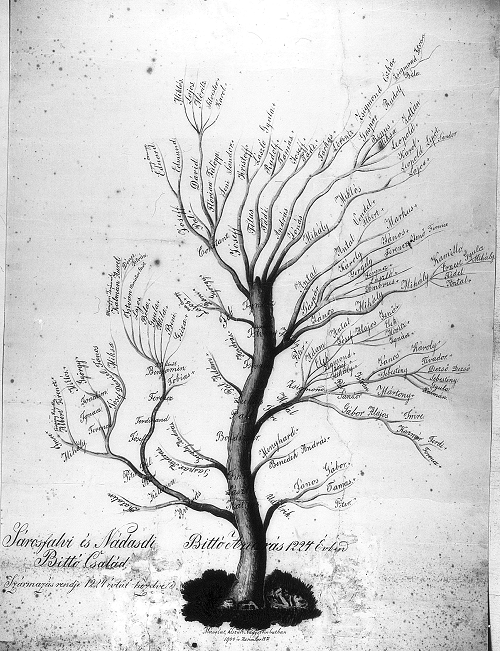
\includegraphics[width=70mm, keepaspectratio]{figures/bitto_csaladfa.png}
\caption{A Bittó család régi típusú családfája.}
\label{fig:bitto_csaladfa}
\end{figure}

Alapvetően a családfák két típusát különböztetjük meg.

\begin{itemize}
 \item Egy meghatározott személy őseit bemutató családfa; ez általában, mint egy fa koronája, felfelé növekszik.
 \item Egy személy (vagy pár) leszármazottait bemutató családfa; formája pont ellentétes az előzőéhez képest, akárcsak a fa gyökérzete, ,,lefelé'' növekszik.
\end{itemize}

Természetesen a fenti két típus kombinációja is elképzelhető, azonban ez ,,offline'' megoldásban nagyon gyorsan kezelhetetlenné és átláthatatlanná válhat. Szoftveres segítséggel azonban akár a bővebb családunk több generációt felölelő teljes családfáját is könnyedén megszerkeszthetjük és karban tarthatjuk. Sőt, akár olyan (pl. multimédiás) anyagokat tárolhatunk a családfában szereplő személyek mellett szinkronban, amelyek további információkkal és emlékekkel tudják teljessé tenni az ábrázolt család (akár a saját családunk) történetét.
